\documentclass[dissertation.tex]{subfiles}
\begin{document}

\chapter{A Preoperative Molecular Prognostic for Pancreas Cancer}
\label{chap:nomogram}

\emph{Thesis: A preoperative prognostic tool for pancreas cancer can be developed to discriminate good between and poor prognosis patients more reliably than current methods.}

\paragraph{Summary}
For those patients fortunate enough to be diagnosed with a resectable tumour, surgical removal of the primary cancer is the best first-line therapy for pancreas cancer.  However, the significant morbidity associated with pancreas cancer resection makes it cruicially important to only operate on the patients who will derive a net benefit from the procedure.  Identifying just those patients who will respond to resection remains a serious challenge in pancreas cancer treatment: current criteria to select patients for resection perform poorly, and consequently many patients undergo a complex procedure, with serious effects on future quality of life, for little benefit.  Tumour biomarkers have the potential to dramatically refine morphology-based staging criteria by supplying a direct readout of tumour biology, and recent technological developments have enabled the preoperative measurement of tissue biomarkers in pancreas cancer.  The ability to measure pancreas cancer tissue biomarker levels preoperatively, combined with the enhanced information on disease state available from tissue biomarkers, finally enables the development of preoperative staging systems that accurately identify pancreas cancer patients for resection.  This chapter details the development and validation of \gls{PCOP}\glsreset{PCOP}, a two-biomarker prognostic tool for resectable pancreas cancer, that is in principle pre-operatively assessable, and can assist in making personalised treatment decisions.


\section{Introduction}
For patients with a resectable tumour and no known metastases, surgical removal of the primary tumour is the current recommended first-line therapy for pancreas cancer, and the only intervention offering the realistic possibility of a cure \cite{Editors2015}.  However, pancreas cancer resection is a major procedure, with the potential for serious complications, morbidity, and reduced quality of life following recovery \cite{Ho2005}.  Due to the substantial negative effects of surgery, the decision of whether or not to perform curative-intent resection should balance the risks of surgery against its expected benefits, for each individual case.

Unfortunately, current practice guidelines recommend that curative-intent surgery be offered to all metastasis-free patients with a resectable tumour, with no consideration of personal benefit \cite{Editors2015}.  This blanket approach to selecting patients for curative resection has proven to be highly inadequate.  Even following pathologically complete tumour removal and adjuvant chemotherapy, more than 70\% of current pancreas ductal carcinoma patients will relapse with, and ultimately succumb to, distant metastases \cite{Barugola2007}.  These occult metastases must have been present prior to removal of the primary tumour, yet were undetectable during initial investigations, and their presence means that any curative-intent resection was futile.  As a result, the majority of `curative' resections that are undertaken based on current selection criteria are performed on patients with occult metastases, have no hope of actually effecting a cure, and would not have been undertaken at all if the presence of metastatic disease had been known prior to surgery.  Better methods to select patients for resection are urgently needed.

\mpfatal{Add something about prognostics as intuitive selection / guidance tools here.  Especially in a relative context.}

A number of pancreas cancer grading and schemes and prognostic tools have been described, but inconsistent performance, or a reliance on information that can only be known post-operatively, limits their use in pre-operative decisions.  The level of serum \gls{CA-19-9} is a well-characterised biomarker of pancreas cancer, with high levels correlating with increased tumour burden, lower probability of resectability, increased post-resection recurrence, and worse prognosis \cite{Kim2011, Ballehaninna2012, Barugola2007, Lundin1994}.  \Gls{CA-19-9} levels are easily determined pre-operatively, but the use of this marker is complicated by a lack of consensus on threshold concentrations, the elevation of \gls{CA-19-9} levels by a number of conditions other than pancreas cancer, and the complete absence of this marker in approximately 10\% of the general population \cite{Ballehaninna2012}.  Additionally, although \gls{CA-19-9} levels are statistically associated with post-resection recurrence by distant metastasis, a very low \gls{PPV} renders the biomarker unhelpful when deciding whether or not to resect \cite{Kim2011}.

The current standard prognostic tool for pancreas cancer is the \gls{MSKCC} nomogram \cite{Brennan2004}, which integrates a number of \glspl{CPV} to arrive at point estimates of survival post-resection.  Unfortunately, its clinical utility is small: as it relies on information that is only available following resection, the \gls{MSKCC} nomogram is only useful in a post-operative context, and cannot assist in pre-operative decisions to resect.  This severely limiting reliance on postoperative variables is made necessary by the fact that all strong classical prognostic factors in pancreas cancer (such as lymph node infiltration, resection margin status, or histological grade \cite{Bilici2014}) can only be reliably measured following resection.  Any prognostic tool for pancreas cancer that relies heavily on classical \glspl{CPV} will very likely share this same reliance on post-operative variables, and so an effective pre-operatively assessable prognostic will need to shirk classical \glspl{CPV}, and leverage novel pre-operative measures of prognosis.
%The \gls{MSKCC} nomogram also provides relatively little information to the user, supplying only an aggregate risk score and survival probabilities at three fixed times, with no indication of prediction confidence or prognosis over the full disease course.  These technical limitations are a consequence of the simple construction of the \gls{MSKCC} nomogram, so chosen to facilitate hand calculation.  With the widespread availability and use of portable computers and smart phones today, limiting performance for the sake of allowing hand calculation is no longer necessary, and return of far richer prognostic information is straightforward.

Levels of tissue biomarkers directly reflect cellular state, and thus have the potential to predict cancer behaviour far more reliably than macroscopic \glspl{CPV}.  Given that most pancreas cancer patients who undergo curative resection quickly recur due to occult metastases, biomarkers of metastasis have the potential to identify those patients who are likely to already have occult metastatic disease at the time of surgery, and thus better inform the decision to resect.  Two such biomarkers of metastasis are the cancer cell levels of the \gls{EMT}-related S100A2, and S100A4 proteins, both of which are strongly predictive of outcome following resection, and appear to reflect the presence of a pro-metastatic invasive phenotype in the cancer \cite{Biankin2008, Tsukamoto2013, Lee2014}.  Despite this promise, these tissue biomarkers have to date only been assessed in bulk tissue samples collected during surgery, and their utility, or even measurability, in a pre-operative setting, is untested.

Recent techological developments have made possible the pre-operative measurement of tissue biomarkers during \gls{EUS}, a routine diagnostic modality for pancreas cancer.  \Gls{IHCal} staining has been successfully performed on \gls{FNA} biopsies of pancreas neoplasms collected during \gls{EUS} \cite{Popescu2012, Salla2009, Stelow2005}, and in principle \gls{EUS}-\gls{FNA}-\acrshort{IHCry} could form the basis of a routine pre-operative biomarker measurement methodology in pancreas cancer.  This proposed biomarker measurement approach utilises only techniques that are commonly available in pancreas cancer treatment centres, and thus has the potential to be rapidly integrated into current diagnostic workflows, should biomarker measurements prove to be clinically valuable.

The nexus of known biomarkers of metastatic behaviour, new pre-operatively applicable techniques to measure these biomarkers, and multiple large, clinically annotated cohorts of resected pancreas cancer, presents an opportunity to address the pressing need for better criteria to select patients for pancreas cancer resection.  As part of the \gls{APGI}, as well as other work, the group has collected tissue measurements of S100A2 and S100A4 biomarkers, and detailed patient follow-up, for a large number of cases of pancreas cancer from a range of independent cohorts.  These cases will be used to develop \gls{PCOP}, a tool to predict outcome following resection, using tissue levels of S100A2 and S100A4 as major prognostic factors.  This initial version of \gls{PCOP} is based on biomarker measurements made on tissue collected during resection, and thus will not be directly applicable pre-operatively.  However, pilot study data will be used to demonstrate that levels of S100A2 and S100A4 measured by pre-operative \gls{EUS}-\gls{FNA}-\acrshort{IHCry} correlate well to tissue levels of the biomarkers measured on operative specimens, indicating that a more refined version of \gls{PCOP} trained on pre-operative data will be equally effective.

The majority of pancreas cancer resection procedures today are performed on patients who should never have been offered surgical resection at all.  These patients have undetected metastases at the time of surgery, and will derive little benefit from a major operation, that has serious impacts on quality of life.  Current tools for patient staging and estimation of prognosis are either ineffective at identifying patients at risk for occult metastases, or only applicable post-operatively, and so cannot be used to inform the decision of whether or not to resect.  Tissue biomarkers of metastatic potential might identify, pre-operatively, those patients who have a high likelihood of metastatic disease, greatly assisting disease management decisions.  This metastasis prediction can be integrated with other clinical variables to yield personalised estimates of prognosis over time, that are well-suited to .  This chapter describes the use of pre-operatively assessable variables, including biomarker measurements, to create \gls{PCOP}, a tool that produces estimates of prognosis.  \Gls{PCOP} provides a natural way to show the influence of risk factors on a patient's personalised prognostic path, and thus can assist in making treatment decisions appropriate for each individual pancreas cancer patient.

\section{Results}
Data from the large, retrospectively-acquired \gls{NSWPCN} cohort were used to derive \gls{PCOP}, a tool to predict the survival of pancreas cancer patients following curative-intent resection.  Discrimination and calibration of \gls{PCOP} were verified on two independent surgical cohorts.  Data from an \gls{EUS}-\gls{FNA}-\acrshort{IHCry} pilot study established that pre-operatively assessed tissue biomarker levels reflected measurements from operative biopsies, and therefore that \gls{PCOP} could be translated to a pre-operative decision setting.

\subsection{Prognostic variables and biomarkers}
As the aim was to develop a prognostic predictor that could be applied pre-operatively, only the small subset of traditional \glspl{CPV} that were deemed to be measurable prior to resection were considered.  These variables were: patient sex and age at diagnosis, tumour location (dichotomised as head of pancreas vs other location), and size of the tumour's longest pathological axis.  Pre-operative measurements of tumour size (for example, by \gls{CT} X-ray or \gls{EUS}) were not available in the training and validation sets, and were approximated by post-operative measurements during the development and testing of this nomogram.  \mpfatal{For the disc: Although the correlation between \gls{CT} and \gls{EUS} estimates of tumour size, and actual size upon resection, is respectable \cite{Arvold2011}, full clinical validation of this prognostic's use in a pre-operative setting will require ...}

The dichotomised tissue levels of two pre-operatively assessable biomarkers, S100A2 and S100A4, were considered when building the prognostic tool.  These biomarker levels were measured by \gls{IHCry} on tissue collected during resection, and thus could potentially be 

The implications of these approximations for the prognostic tool developed here, as well as for future work, are considered in the discussion.

\mpfatal{Stuff on biomarkers.  Specifically, why I didn't use CA-19-9.}

\subsection{Cohorts and Characteristics}
General characteristics of the \gls{NSWPCN}, Glasgow, and Dresden cohorts are summarised in \tref{tab:nomo-cohort-characteristics}.\mpfatal{TODO.  Waiting on DC's data.}

\begin{table}[h]
\centering
\caption[Characteristics of patient cohorts]{Characteristics of the \gls{NSWPCN} training cohort, and the Glasgow and Dresden validation cohorts.  Ordinal variables are shown as median, with quartiles in parentheses.  Categorical variables for which percentages do not add up to 100\% indicate the presence of minor unlisted categories.}\label{tab:nomo-cohort-characteristics}
\begin{tabular}{@{}lllll@{}}
\toprule
Characteristic         &         & NSWPCN       & Glasgow      & Dresden      \\ \midrule
Number of patients     &         & xx           & xx           & xx           \\
Gender                 & Male    & xx\%         & xx\%         & xx\%         \\
Age at diagnosis       & (years) & xx (xx - xx) & xx (xx - xx) & xx (xx - xx) \\
Tumour location        & Head    & xx\%         & xx\%         & xx\%         \\
Size of longest axis   & (mm)    & xx (xx - xx) & xx (xx - xx) & xx (xx - xx) \\
S100A2 positive        &         & xx (xx - xx) & xx (xx - xx) & xx (xx - xx) \\
S100A4 positive        &         & xx (xx - xx) & xx (xx - xx) & xx (xx - xx) \\
Excision margin status & R0      & xx\%         & xx\%         & xx\%         \\
                       & R1      & xx\%         & xx\%         & xx\%         \\
                       & R2      & xx\%         & xx\%         & xx\%         \\
Node involvement       &         & xx\%         & xx\%         & xx\%         \\
Disease-specific death &         & xx\%         & xx\%         & xx\%         \\
Length of follow-up    & (days)  & xx (xx - xx) & xx (xx - xx) & xx (xx - xx) \\ \bottomrule
\end{tabular}
\end{table}

\subsection{Prognostic model building and selection}
Candidate prognostic models were constructed on the \gls{NSWPCN} training data by iterative model fitting, evaluation, and refinement.  To guard against overfitting caused by this iterative process, the \gls{NSWPCN} cohort was randomly split once into model building and testing sets.  All model fitting and refinement described below was performed on the model building set, to yield three final candidate prognostic predictors.  The performance of each of these three predictors was then assessed on the model test set, and the most parsimonious high-performing model was chosen as the final prognostic predictor, for subsequent external validation.

\paragraph{Model functional form and expanded terms}
The \gls{CPH} framework was used to assess functional form for the two continuous covariates: age at diagnosis, and maximum pathological axis size.  \gls{LOESS} smooths of martingale residuals \cite{Therneau1990} indicated a possible weak U-shaped relationship for age at diagnosis (\fref{fig:nomo-funcform-age}), and a knee-shaped form for size (\fref{fig:nomo-funcform-size}), with the knee at approximately $0$ in median-centered units.  In subsequent fits these forms were modelled by adding a quadratic term for centered age at diagnosis, and a $\mbox{size}_+$ ramp term for centered axis size.  The original set of five linear prognostic terms, plus the two additional nonlinear terms, was denoted the expanded term set.

\begin{figure}
\centering
  \subbottom[Patient age (centered)]{
    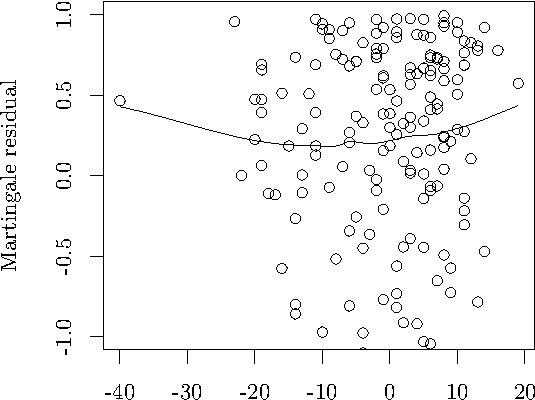
\includegraphics[width=.45\linewidth]{analysis/nomogram/figure/05-eda-func-form-age-2}
    \label{fig:nomo-funcform-age}}
  \subbottom[Tumour size (centered)]{
    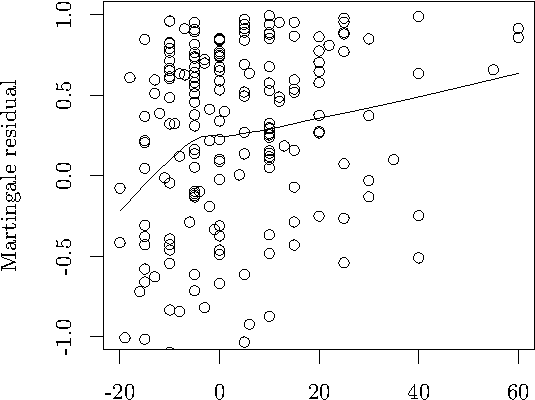
\includegraphics[width=.45\textwidth]{analysis/nomogram/figure/05-eda-func-form-size-2}
    \label{fig:nomo-funcform-size}}
\caption[Prognostic predictor functional forms]{Smoothed Cox model martingale residual plots indicate hazard relationships that are approximately quadratic for centered age (panel a), and piecewise linear for centered tumour size (panel b).  For clarity, plots have been restricted to the residual range $[-1,1]$.}
\label{fig:nomo-funcform}
\end{figure}

\paragraph{Proportional hazards assumption}
A Grambsch-Therneau test \cite{Grambsch1994} on the \gls{CPH} model fit using all expanded terms indicated that patient sex violated the \glspl{PH} assumption (P = TODO, \fref{fig:nomo-ph-plot-sex}) -- in other words, the two sexes had significantly different baseline hazard shapes.  To account for this effect, all subsequent models were stratified by patient sex, so that the survival of male and female patients was modelled by two different baseline hazard functions.  A repeated Grambsch-Thernau test on the stratified model indicated no further significant violations of the \gls{PH} assumption (global P = TODO).

\begin{figure}
\centering
  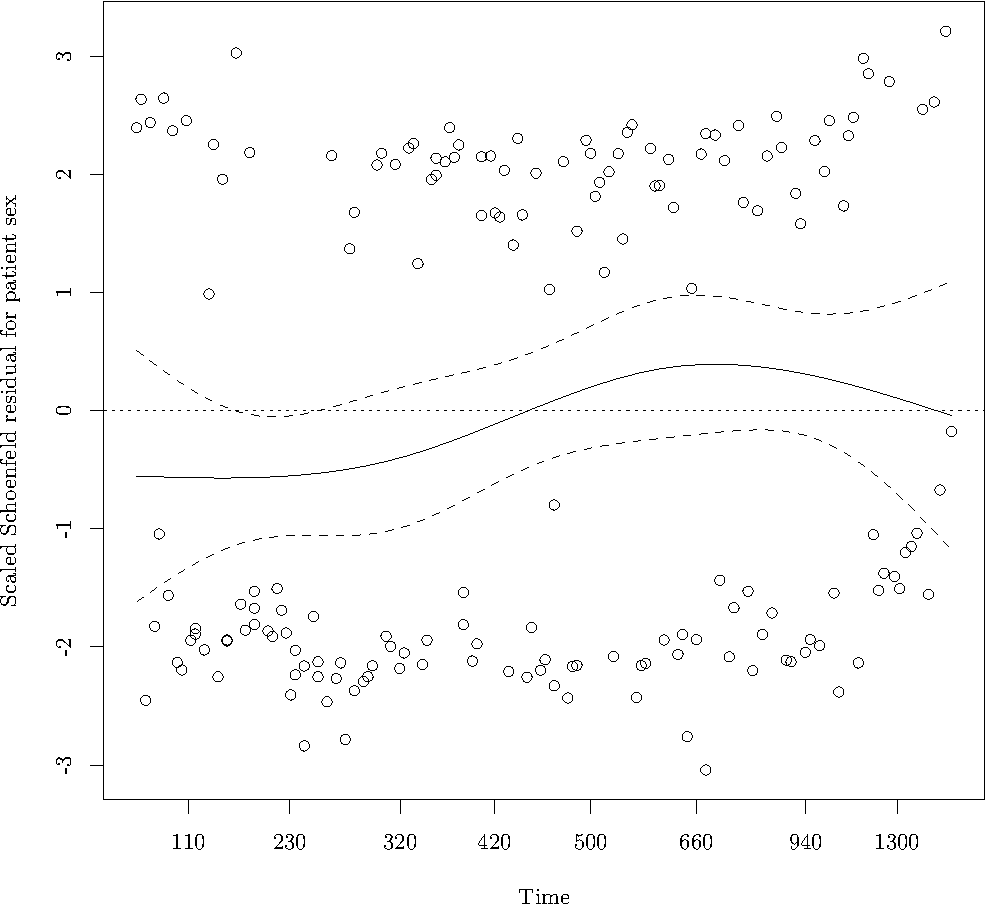
\includegraphics[width=.7\linewidth]{analysis/nomogram/figure/05-eda-ph-check-full-sexplot-1}
  \caption[Baseline hazard forms differ between patient sexes]{Baseline hazard differs between patient sexes.    
  A natural spline smooth of scaled Schoenfeld residuals for patient sex has a slope obviously differing from zero, suggesting that the baseline hazard forms differ between the two sexes, and that the combined data violates the \acrshort{PH} assumption of Cox regression.  Individual residuals are displayed as points, the natural spline smooth ($\mbox{df}=4$) as a solid line, and approximate $\pm 1\ \mbox{SE}$ bounds as dashed lines.}
\label{fig:nomo-ph-plot-sex}
\end{figure}

\paragraph{Variable selection}
Genetic selection was used to identify a model with optimal \gls{BIC} from the set of all \gls{CPH} models that use any combination of the expanded terms.  Models with interactions between terms of up to degree two were considered, and a marginal term constraint was enforced, to ensure that interaction effects were only present in the model specification if the associated main effects were also.  Stratification of baseline hazard by patient sex was used in all models.  The identified optimal \gls{CPH} model used three variables: tumour size (linear term only), S100A2 status, and S100A4 status, in addition to the sex stratum.  This model was also identified by stepwise backward selection for optimal BIC, starting from the marginal \gls{CPH} fit using all expanded terms.  The final \gls{BIC}-selected set of prognostic terms (tumour size linear term, S100A2 binary status, S100A4 binary status, and a patient sex stratum) was denoted the reduced term set.

\paragraph{Model CP1}
A final prognostic \acrshort{CPH} regression model was fit to the \gls{NSWPCN} model building data using only the reduced term set; this model was termed CP1.  CP1 did not violate the \gls{PH} assumption by the Grambsch-Therneau test (global P = TODO).  Model residuals were inspected to identify possible outlier patients, and assess overall fit stability.  Deviance residuals indicated no egregious outlier patients, and DFBETAS indicated TODO influential patients with $|\mbox{DFBETAS}_{i,j}| > \frac{2}{\sqrt{n}}$, where $n = TODO$.  TODO: Stuff on these outliers.  Predictions from model CP1 were broadly concordant with stratified \gls{KM} estimates across all covariate subgroups, indicating no serious lack of fit of the model (\fref{fig:nomo-cp1-gg1-fitplot}).

\paragraph{Model GG1}
Semiparametric Cox \gls{PH} models such as CP1 provide a convenient framework for covariate testing and model diagnostics, but their unspecified baseline hazard term significantly complicates their use as prognostic predictors: patients can only be ranked by relative hazard, and absolute estimates of survival probabilities are unavailable.  Although it is possible to approximate the baseline hazard in the Cox model, a more robust alternative is to use fully parametric models, in which the baseline hazard distribution is explicity specified.  The advantages of parametric models in terms of robustness and interpretability are offset by their more stringent assumptions: if the chosen baseline distribution is unsuited to the particular data to be fit, predictions from parametric models can be very poor.  Given the potential benefits of parametric models for survival prediction, a parametric alternative to model CP1 was developed, and its fit assessed.  This parametric model was termed GG1.

Model GG1, employing a \gls{GG} survival distribution \cite{Cox2007}, was fit to the \gls{NSWPCN} model building data by maximum likelihood.  Guided by the model functional form and baseline hazard stratification indicated by the Cox model diagnostics, the \gls{GG} distribution location parameter $\beta$ was made linearly dependent on all terms in the reduced set, but the shape parameters $\sigma$ and $\lambda$ were modelled as dependent on patient sex only.  The goodness of fit of GG1 was investigated by examination of residuals, and graphical assessment of prediction accuracy.  Deviance and DFBETAS residuals indicated no extreme outliers or unduly influential samples, and GG1 survival predictions matched empirical \gls{KM} estimates to within error across a range of covariate values and times (\fref{fig:nomo-cp1-gg1-fitplot}).

\begin{figure}
\centering
  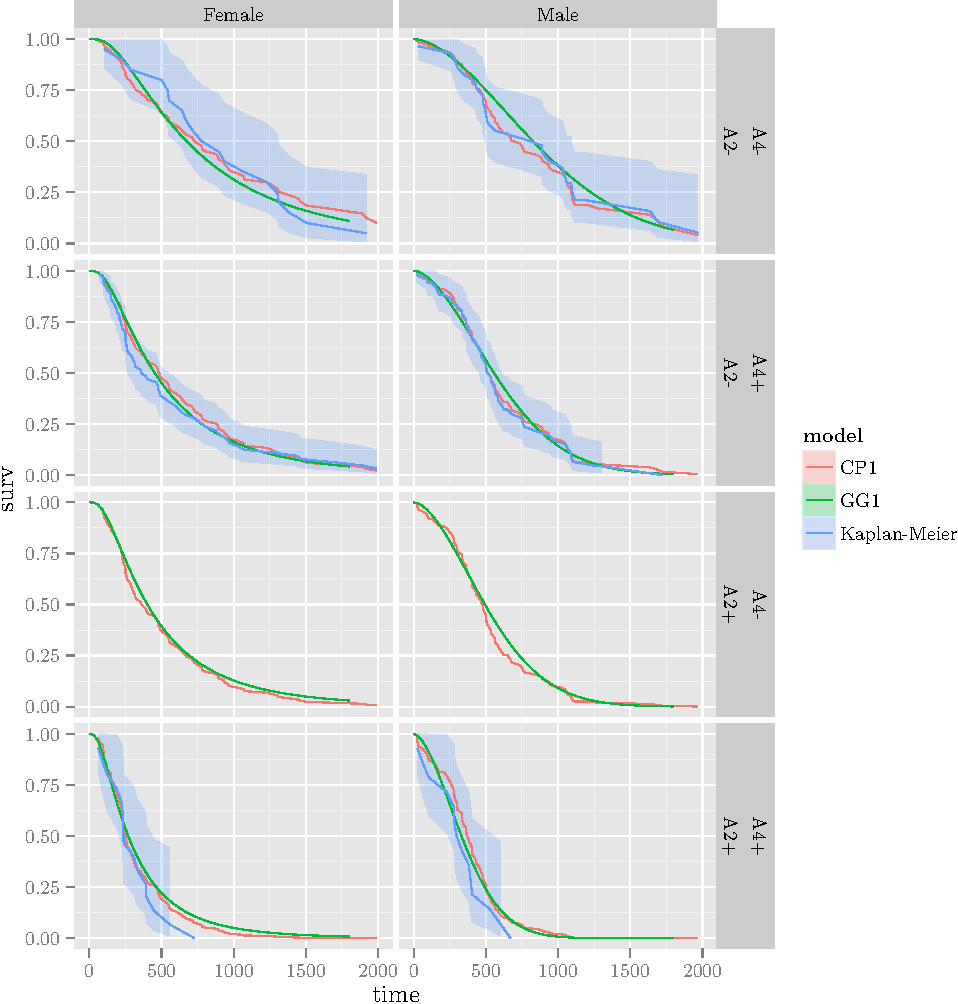
\includegraphics[width=.7\linewidth]{analysis/nomogram/figure/05-final-fit-assessment-4-2}
  \caption[Model survival predictions agree with stratified \acrshort{KM} estimates]{Model survival predictions agree with stratified \gls{KM} estimates.  \gls{KM} estimates of survival probability for each combination of patient sex and biomarker status are shown as solid blue lines, with 95\% confidence intervals indicated by blue ribbons.  Estimates of survival probability generated by both models CP1 (red) and GG1 (green) broadly followed the form of the \gls{KM} estimator, and lay within its bounds at all times.  Predictions were made using the \gls{NSWPCN} model building set, and so these plots illustrate model goodness-of-fit, but cannot indicate possible overfitting.  \gls{KM} traces for the S100A2 positive, S100A4 negative group were omitted, as there were insufficient patients in this group for reliable \gls{KM} estimates to be available.}
\label{fig:nomo-cp1-gg1-fitplot}
\end{figure}

\paragraph{Model RSF}
Regression models like CP1 and GG1 are familiar and readily interpretable, but are heavily dependent on the analyst identifying appropriate variables and functional forms.  Ensemble tree models such as random forests \cite{Breiman2001} naturally and automatically model nonlinearity and arbitrary level interactions, and are tolerant of large numbers of irrelevant or collinear variables, albeit at the cost of very poor interpretability, and large data and computational requirements.  Random forests have been adapted to model censored data \cite{Ishwaran2008}, and can provide an alternative prognostic predictor that is distinct in behaviour from CP1 and GG1, and may be able to exploit data structure not leveraged by these more classical models.

To investigate whether tree ensemble models could provide improved performance over classical approaches, a random survival forest model, termed RSF, was fit to the \gls{NSWPCN} model building data.  In contrast to CP1 and GG1, which used the reduced set of terms as covariates, RSF was supplied all preoperatively-assessable variables as candidate predictors.

\paragraph{Model selection}
Predictive performance of the three prognostic models (CP1, GG1, and RSF) was compared on the holdout \gls{NSWPCN} model test set, to select a single high-performing parsimonious model for external validation.  For each model, prediction accuracy over time was assessed by the Brier score for censored data \cite{Graf1999}, and overall accuracy was measured by the \gls{IBS}.  All predictors were also compared against a no-information control predictor, formed as the \gls{KM} estimate of the marginal survival function in the \gls{NSWPCN} model building set.  This no-information estimate, here denoted KM0, is the optimal survival predictor in the absence of any prognostic information or patient stratification; the prognostic models developed here must at least outperform KM0 to be of any clinical utility.

\begin{figure}
\centering
  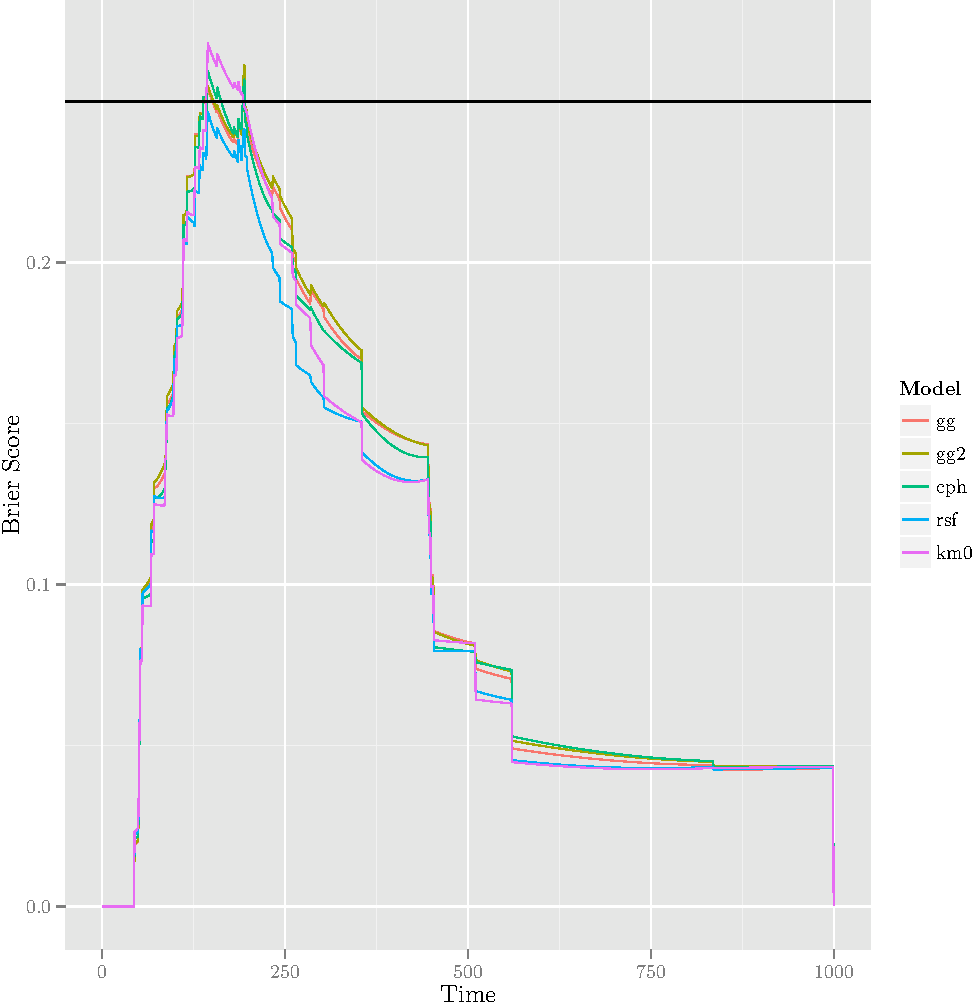
\includegraphics[width=.7\linewidth]{analysis/nomogram/figure/05-model-selection-bs-paths-1}
  \caption[Brier score paths for candidate models on holdout data]{Brier score paths for candidate models on the holdout \gls{NSWPCN} model test set.  All models outperformed the no-information KM0 trace from approximately 100 days to 600 days post-diagnosis, and no strong differences were apparent between candidate models.}
\label{fig:nomo-brier-paths}
\end{figure}

Traces of the Brier score over time indicated that all models produced survival estimates superior to KM0 from approximately 100 days to 600 days post-diagnosis (\fref{fig:nomo-brier-paths}).  The performance of the models was similar, with RSF displaying slightly higher error rates at longer follow-up times, and models CP1 and GG1 demonstrating comparable performance.  Bootstrapped differences in \gls{IBS} between KM0 and each prognostic model further highlighted that although all competing models were superior to KM0, the models displayed statistically similar predictive performance on the test set (\fref{fig:nomo-ibs-delta}).  As there was no substantial difference in performance between the prognostic models, the simplest model GG1 was selected for external validation.

\begin{figure}
\centering
  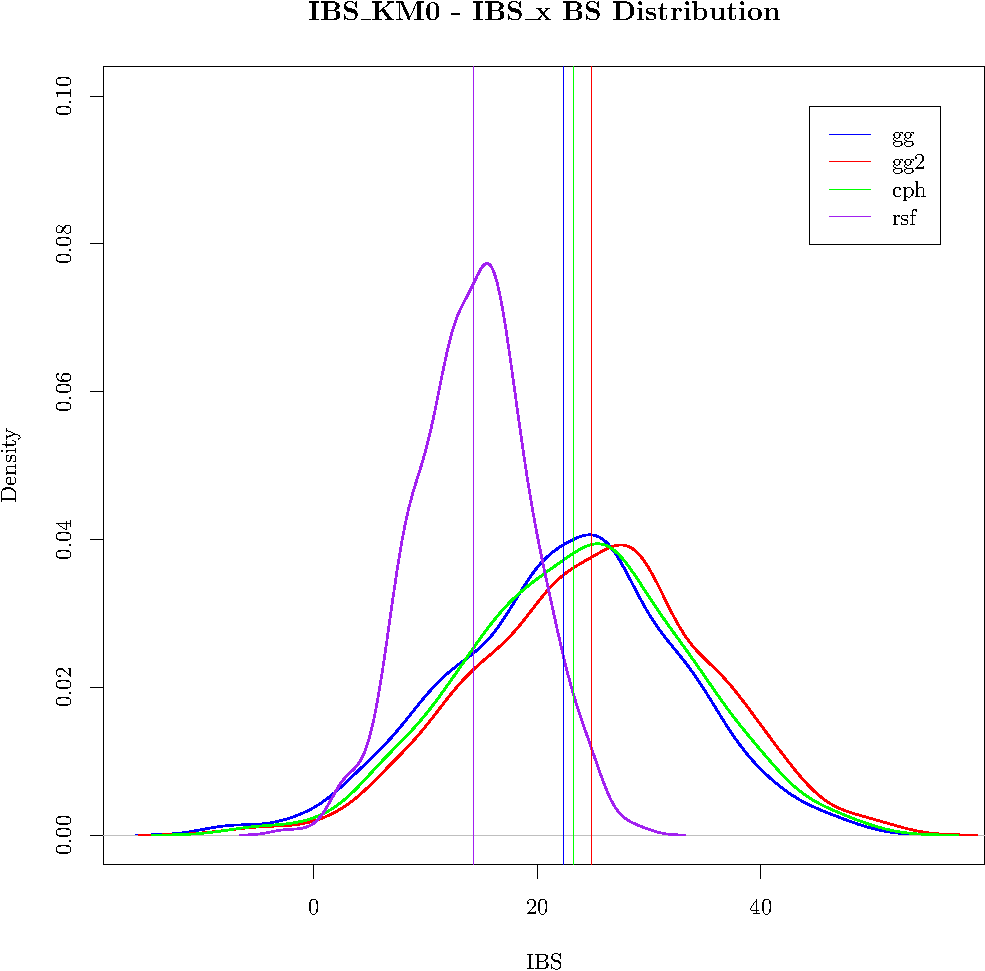
\includegraphics[width=.7\linewidth]{analysis/nomogram/figure/05-model-selection-ibs-3}
  \caption[Bootstrapped differences in \acrshort{IBS} between candidate models and KM0]{Distribution of bootstrapped differences in \gls{IBS} between candidate models and null-model KM0.  For each of 500 bootstrap draws from the \gls{NSWPCN} holdout model test data, the difference between the \gls{IBS} of a candidate model, and the \gls{IBS} of KM0, was calculated as $\Delta \mbox{IBS}_{\mbox{Model}} = \mbox{IBS}_{\mbox{KM0}} - \mbox{IBS}_{\mbox{Model}}$.  The smoothed distributions of $\Delta \mbox{IBS}_{\mbox{Model}}$ are shown here for each candidate model.  All models predicted outcome significantly better than KM0, but beyond that had statistically similar performance.}
\label{fig:nomo-ibs-delta}
\end{figure}

%\paragraph{Summary}
%Exploratory analysis on the training \gls{NSWPCN} cohort data indicated that a BIC-optimal \gls{CPH} fit was achieved by the following model: $T \sim \mbox{Age} + \mbox{S100A2} + \mbox{S100A4} + \mbox{strata}(\mbox{Sex})$.  There was no significant evidence for nonlinear effects in any examined variables, or for any interactions up to degree two.  Male and female patients appeared to have significantly different baseline hazards, a feature that was modelled by stratifiying by patient sex.  The performance of \gls{CPH} and parametric predictors that followed the above model form, and a general \gls{RSF} predictor, were compared on holdout data.  The \gls{RSF} predictor was inferior to the \gls{CPH} and parametric models, which were equivalent.  The parametric model, termed GG1, had the optimal combination of performance and parsimony, and was selected for external validation.

\subsection{External validation}

\subsection{Web tool}


%* Summary of analysis
%* Variables that are both available and reasonably pre-operatively assessable:
%  # Patient:   Age, Sex
%  # Imaging:   Size, Location (head vs tail)
%  # Biomarker: A2, A4, CA-19-9 (thresh 100 U/mL)
%* Cohort subsetting and characteristics (all of them)
%* Exploration.
%  # Functional forms.  Martingale residual smooths of marginal model.
%  # Perform CPH fit of marginal model using identified forms, examine violations of CPH.  Identify Sex and A4 as violators.  Re-fit with strata to resolve.  Probably just describe this step as a reason for stratification by Sex, A4.
%* All-subsets search for best model, including interactions.
%

TODO: In app, show +/- margin curves, to guide surgeons as to benefit from aggressive surgery.


\subsection{Cohort characteristics}
\label{subsec:nomo-results-cohort}

\subsection{Development of a preoperative prognostic model}

\subsection{Validation of the prognostic model}
Intro here on disc \& calib.  Also describe cohorts briefly.
\subsubsection{Discrimination}
\subsubsection{Calibration}

\subsection{Web tool TODO -- better name}

\section{Discussion}

\section{Methods}
\subsection{Cohort recruitment and ethics}
\label{subsec:nomo-methods-cohort}

\end{document}
